\section{Communication Library}\label{sec:runtime}

implementation software layer

3種:one sided, collective, atomic. このうちcollectiveとatomicはMPIの機能をそのまま使う。それ以上の工夫はない。one sidedはallocate/freeとput/getと同期。lower-level通信層のバリエーションを吸収するライブラリ層を設けた。階層の図。

\begin{figure}[tbh]
  \begin{center}
  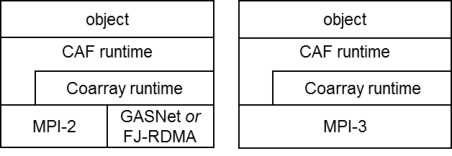
\includegraphics[scale=1.0]{figs/layer.pdf}
  \caption{Software Layer}\label{fig:layer}
  \end{center}
\end{figure}

cf.\ air:/Users/iwashita/Desktop/coarray/Project\_Coarray/coarray implement 6-1.docx 他



次元の概念とcontiguityを上位層で解決するため結果的に必要なインタフェースは少なくなった。表

\begin{table}
 \begin{center}
  \caption{使用したCoarrayランタイムインタフェース(未公開機能関連を除く)}
  \begin{tabular}{|l|l|}
\hline
割付け・解放と登録
& 1. \verb|_XMP_coarray_malloc_image_info_1|\\
& 2. \verb|_XMP_coarray_malloc_info_1|\\
& 3. \verb|_XMP_coarray_malloc_do|\\
& 4. \verb|_XMP_coarray_regmem_do|\\
& 5. \verb|_XMP_coarray_lastly_deallocate|\\
\hline
片側通信
& 6. \verb|_XMP_coarray_shortcut_get|\\
& 7. \verb|_XMP_coarray_shortcut_put|\\
\hline
同期
& 8. \verb|xmp_sync_all|\\
& 9. \verb|xmp_sync_image|\\
& 10 \verb|.xmp_sync_images|\\
& 11 \verb|.xmp_sync_images_all|\\
& 12 \verb|.xmp_sync_memory|\\
\hline
atomic通信
& 13 \verb|._XMP_atomic_define_0|\\
& 14 \verb|._XMP_atomic_define_1|\\
& 15 \verb|._XMP_atomic_ref_0|\\
& 16 \verb|._XMP_atomic_ref_1|\\
\hline
問合せ
& 17 \verb|.xmp_all_num_nodes|\\
\hline
エラー処理
& 18 \verb|._XMP_fatal|\\
\hline
  \end{tabular}
 \end{center}
\end{table}

